\section{Théorie}

Lorsqu'un courant intense traverse un transformateur composé de nombreuses spires il se crée une induction magnétique dont l'intensité s'exprime par l'équation:
\begin{equation}
    B = \mu_0 I \frac{N}{L} = \mu_0 \frac{V_i}{R} \frac{N}{L}
    \label{eq:B_I}
\end{equation}
Dans laquelle \(B\) est l'intensité de l'induction magnétique considérée, \(I\) est le courant qui traverse le transformateur, \(N\) le nombre de spires du primaire du transformateur et \(L\) la longueur du transformateur \cite{assistant}. La deuxième équation est obtenue en sachant que l'intensité du courant est constante dans tout le circuit et par la loi d'Ohm \(V_i = RI\) avec \(R\) la résistance placée à l'entrée du transformateur et \(V_i\) la tension mesurée à ses bornes.

De plus dans un matériau donné la relation entre l'induction magnétique et le champ magnétique présent est donné par:
\begin{equation}
    B = \mu_0 (\chi_m + 1) H = \mu_0 \mu_r H
    \label{eq:B_H}
\end{equation}
Avec \(B\) et \(H\) l'induction et le champ magnétique, \(\chi_m\) la susceptibilité magnétique du matériau et \(\mu_r = \chi_m + 1\) sa perméabilité relative \cite{notice}. La perméabilité absolue du vide est exactement définie par \(\mu_0 = 4\pi \times 10^{-7}\) \si{\volt\second \per\ampere\per\meter}.

De la même manière que le primaire du transformateur crée une induction magnétique, cette induction magnétique produit également un courant dans le secondaire qui sera proportionnelle par la loi d'Ohm à la tension mesurée à sa sortie. Ainsi il est donc possible d'écrire une relation de proportionnalité en définissant une constante \(\alpha\) telle que:
\begin{equation}
    V_f = \beta V_i = \alpha \mu_r V_i
    \label{eq:Vi-Vf}
\end{equation}
Avec \(\beta\) le coefficient de proportionnalité.

En combinant les équations \autoref{eq:B_I} et \autoref{eq:B_H} il est possible de trouver que:
\begin{equation}
    H = \frac{N}{\mu_r L} \frac{V_i}{R}
    \label{eq:calibr_H}
\end{equation}
Et avec la relation entre \(V_i\) et \(V_f\) donné par l'\autoref{eq:Vi-Vf} cela donne également:
\begin{equation}
    B = \mu_0 \frac{N}{L} \frac{1}{\alpha \mu_r} \frac{V_f}{R}
    \label{eq:calibr_B}
\end{equation}

De plus l'\autoref{eq:B_H} permet de conclure que pour le vide \(\mu_r = 1\) et donc \(V_f = \alpha V_i\) pour le vide. Ainsi il faut prendre la régression linéaire des mesures sans échantillon pour le système étudié pour connaître \(\alpha\). Il est ensuite possible de trouver la valeur de \(\mu_r\) en connaissant les coefficients de proportionnalité seulement des tensions qui sont plus simples à mesurer que des inductions et champs magnétiques:
\begin{equation} 
    \mu_r = \frac{\beta}{\alpha}
    \label{eq:mu_r}
\end{equation} 


Les matériaux peuvent se classifier par leur comportement magnétique. Les matériaux diamagnétiques possèdent une perméabilité au magnétisme inférieure à celle du vide car pour ces matériaux \(\chi_m < 0 \Rightarrow \mu_r < 1\). Ceux paramagnétiques possèdent des moments magnétiques internes les rendant plus susceptible à l'induction magnétique avec \(chi_m > 0\). Finalement les matériaux ferromagnétiques présentent des interactions entre ces moments magnétiques internes qui restent même après la disparition d'un champ magnétique créant ainsi un phénomène d'hystérèse.

Les cycles d'hystérèse magnétique présentent deux couples de valeurs caractéristiques. Le premier est le champ \(H_S\) et l'induction \(B_S\) magnétiques de saturation qui correspondent au niveau de magnétisation maximal du matériau considéré. Au-delà de ce champ magnétique la valeur de l'induction présente dans le matériau n'augmentera plus. Le deuxième couple de valeurs est l'induction rémanent \(B_r\) et le champ coercitif \(H_C\). Ils correspondent respectivement à l'induction encore présente au sein du matériau même après la mise à zéro du champ magnétique appliqué et au champ magnétique nécessaire pour venir compenser complètement cette induction rémanente.
\begin{figure}[h]
    \centering
    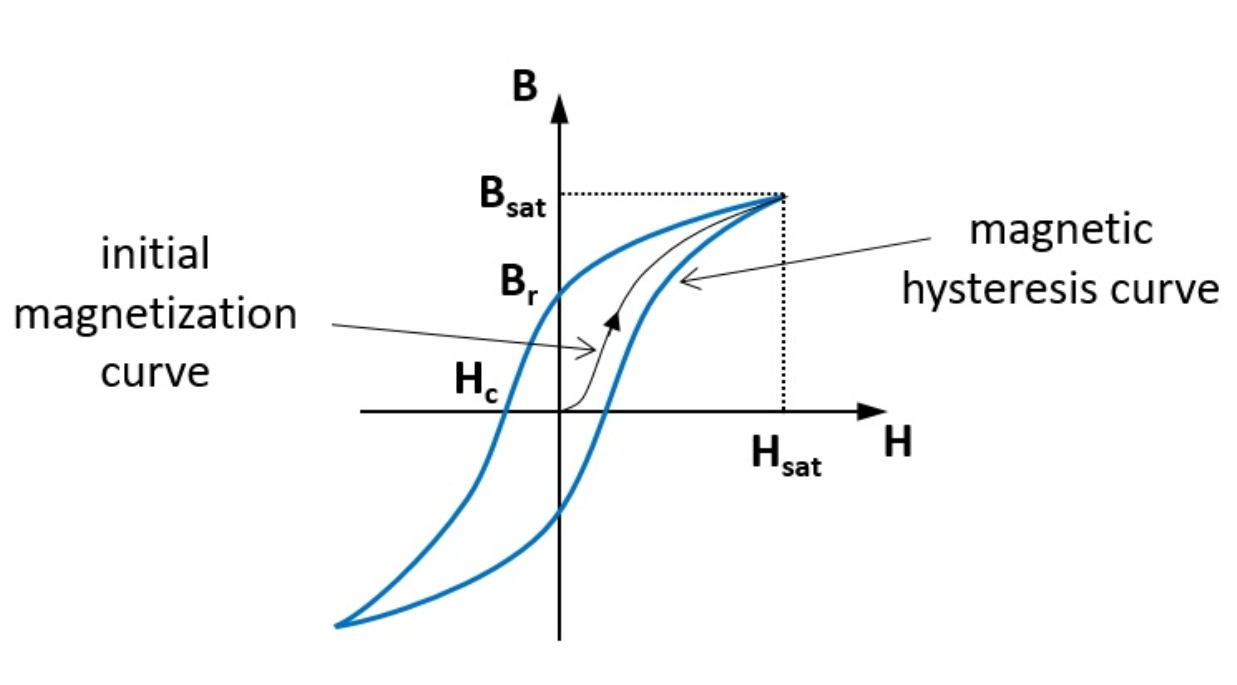
\includegraphics[width=0.7\linewidth]{figures/cycle_hysterese.png}
    \caption{Graphe d'un cycle d'hystérèse magnétique avec ses valeurs caractéristiques \cite{graph_cycle}}
    \label{fig:cycle}
\end{figure}